\label{sota}
\section{MVSR-IDR}
\label{section:idr}
\subsection*{Ανακατασκευή 3D επιφανειών με χρήση Νευρωνικών Δικτύων μέσω πολλαπλών όψεων διαχωρίζοντας τη γεωμετρία και την εμφάνιση}
\par
    Στο πλαίσιο της \enit{3D} ανακατασκευής με την οποία ασχολείται η παρούσα εργασία σημαντική έρευνα είναι αυτή της \enit{Lior Yariv} με τίτλο: Ανακατασκευή επιφανειών με χρήση νευρωνικών δικτύων, μέσω έμμεσων αναπαραστάσεων που προκύπτουν από εικόνες πολλαπλών όψεων, \cite[Multiview neural surface reconstruction by disentangling geometry and appearance]{yariv2020multiview}.
\par
    Τα διαφορίσιμα συστήματα απόδοσης γραφικών, που στοχεύουν την εκμάθηση τρισδιάστατης γεωμετρίας, κυκλοφορούν σε δύο εκδοχές: \enit{differentiable rasterization} και \enit{differentiable ray casting}. Στην παρούσα εργασία, εφόσον μιλάμε για έμμεσες επιφάνειες που αποδίδονται ογκομετρικά και σκοπεύεται ο φωτορεαλισμός επιλέγεται η δεύτερη μέθοδος. Γίνεται περιγραφή συναφών εργασιών για την ανακατασκευή επιφανειών πολλαπλών όψεων και την σύνθεση όψεων με χρήση νευρωνικών δικτύων. 
\par 
     Σε εργασίες όπως \cite{jiang2022sdfdiff} προσεγγίζεται η τιμή της συνάρτησης πολλών μεταβλητών SDF και των κανονικών της διανυσμάτων σε κάθε ογκομετρικό κελί (voxel). Στην εργασία \cite{liu2020dist} χρησιμοποιείται ο αλγόριθμος \enit{sphere tracing} (που αναλύθηκε στο \ref{section:rendering}), σε ένα προ εκπαιδευμένο \enit{DeepSDF} μοντέλο  \cite{park2019deepsdf}. Εκεί, προσεγγίζονται οι παράγωγοι των βαθών ως προς το διάνυσμα εξόδου του \enit{DeepSDF} νευρωνικού δικτύου δηλαδή ως προς το \enit{latent code}του διαφορίζοντας το κάθε ξεχωριστό βήμα του αλγορίθμου του \enit{Differential Sphere Tracing}.  Σε αυτή την εργασία \cite{liu2019learning} χρησιμοποιείται ανιχνευτικό πεδίο για την διευκόλυνση της λειτουργίας του αλγορίθμου ρίψης ακτίνων ώστε να γίνεται εκπαίδευση χωρίς επίβλεψη. Σε αντίθεση με αυτές τις εργασίες, το \enit{IDR} κάνει χρήση διαφορίσιμου σημείου επαφής ακτίνας με επιφάνεια το οποίο έχει ακριβή σε αριθμητική τιμή πρώτη παράγωγο. Επίσης χρησιμοποιείται και το κάθετο διάνυσμα πάνω στο σημείο αυτό με σκοπό την πιο γενικεύσιμη μορφή του μοντέλου εμφάνισης. Τέλος χειρίζεται και κάμερες με θόρυβο. 

     
\subsubsection{Ανακατασκευή από Πολλαπλές Όψεις - Multi-View Synthesis[MVS]} 
\par     
    Κατά την διάρκεια της φωτογράφησης μια εικόνας, η πληροφορία του βάθους χάνεται. Δεδομένης της θέσης και του προσανατολισμού της κάμερας, η κλασσική θεωρία της στερεογραφίας πολλαπλών όψεων (Multi-View Stereo - MVS) έχει μεθόδους \cite{5226635}, \cite{schonberger2016pixelwise}, \cite{campbell2008using}, \cite{tola2012efficient} που προσπαθούν να αναπαράγουν την πληροφορία του βάθους μέσα από την επικάλυψη ή το ταίριασμα χαρακτηριστικών των εικόνων από διάφορες όψεις. Παρ' όλα αυτά, μια μετά-επεξεργασία βάθους \enit{(depth fusion post processing)} \cite{curless1996volumetric}, \cite{merrell2007real} ακολουθούμενη από τον αλγόριθμο ανακατασκευής επιφανειών Poisson \cite{kazhdan2006poisson} είναι απαιτούμενα για την παραγωγή συμπαγούς ανακατασκευής της επιφάνειας. Πρόσφατες μέθοδοι χρησιμοποιούν μια συλλογή σκηνών για την εκπαίδευση βαθιών νευρωνικών μοντέλων, σε επιμέρους εργασίες όπως το \enit{pipeline MVS} (μέσω  αντιστοίχησης χαρακτηριστικών όπως γίνεται στην εργασία \cite{leroy2018shape}), ή με μέθοδο σύντηξης βάθους \enit{(depth fusion)} στις αντίστοιχες εργασίες \cite{donne2019learning}, \cite{riegler2017octnetfusion}. Κάποιες άλλες εργασίες συμβάλλουν σε μια ολοκληρωμένη γραμμή παραγωγής στερεομετρίας από πολλαπλές όψεις \enit{MVS}\cite{huang2018deepmvs}, \cite{yao2018mvsnet}, \cite{yao2019recurrent} και παράγουν αξιόπιστες σαρώσεις \enit{MVS 3D scans}. Πολλές φορές οι παράμετροι της κάμερας βέβαια δεν είναι διαθέσιμες. Σε τέτοιες περιπτώσεις και δεδομένου συνόλου εικόνων από μια συγκεκριμένη σκηνή, υπάρχουν μέθοδοι που τις εξάγουν με \enit{Structure Form Motion} (SFM) με αντίστοιχες μεθοδολογίες \cite{snavely2006photo}, \cite{schonberger2016structure}, \cite{kasten2019algebraic}, \cite{jiang2013global}.  Συγκεκριμένα, εφαρμόζονται για να αναπαράγουν τις κάμερες σε μια αραιή τρισδιάστατη ανακατασκευή εκτιμώντας γραμμικά και τις παραμέτρους των καμερών και μάλιστα η τελευταία χρησιμοποιείται και στην παρούσα εργασία. Τέλος στην εργασία του, ο \enit{Tang Tan} \cite{tang2018ba}, χρησιμοποιεί μια αρχιτεκτονική βαθιού νευρωνικού δικτύου με έναν ολοκληρωμένο διαφορίσιμο νευρωνικό επίπεδο \enit{Bundle Adjustment} \cite{triggs2000bundle} (Δέσμης Προσαρμογής) για να εξάγει μια γραμμική βάση για το βάθος ενός πλαισίου αναφοράς στον χώρο, και τα χαρακτηριστικά από τις γειτονικές εικόνες, ώστε να βελτιστοποιήσει  το βάθος και τις παραμέτρους της κάμερας σε κάθε εμπρόσθιο πέρασμα του δικτύου. 
    
    Σε αντίθεση με αυτές τις εργασίες, το \enit{IDR} εκπαιδεύεται με εικόνες από μια μόνο σκηνή-στόχο, παράγοντας μια ακριβή στεγανή τρισδιάστατη ανακατασκευή επιφάνειας. 
\par
    Όπως ειπώθηκε ήδη, στόχος της συγκεκριμένης εργασίας είναι να επινοήσει ένα ολοκληρωμένο σύστημα όσον αφορά αρχιτεκτονικής βαθιών νευρωνικών δικτύων, το οποίο μπορεί να μάθει τρισδιάστατες γεωμετρίες από \enit{masked} (μάσκα που δείχνει αν καλύπτεται το εξής pixel από το αντικείμενο ενδιαφέροντος) εικόνες 2D  και εκτιμήσεις καμερών, ενώ δεν απαιτεί περαιτέρω επίβλεψη. Στο Σχήμα:\ref{fig:idrnetwork}, απεικονίζεται η συνολική αρχιτεκτονική του δικτύου, η διαφορίσιμη συνάρτηση απόδοσης (\enit{differentiable rendering function} με έμφαση στο διαφορίσιμο σημείο τομής της ακτίνας με την επιφάνεια και την επιστροφή των κλισεων των κάθετων διανυσμάτων, το οποίο αναλύεται και στην μεθοδολογία της διαφορίσιμης εξίσωσης απόδοσης γραφικών βλ.\ref{eq:differentiableRendering})
    \begin{figure}[H]
        \centering
        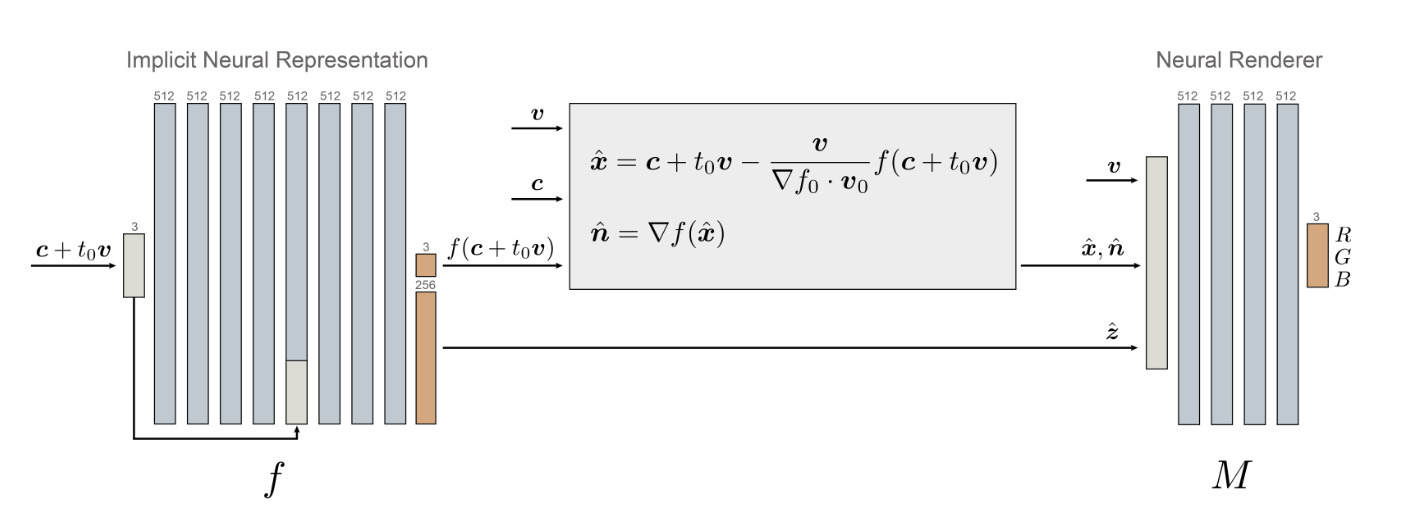
\includegraphics[width = \linewidth]{images/chapter3_img/idr_network_architecture_2.jpg}
        \caption{Συνολικό Δίκτυο IDR, Πηγή \cite{yariv2020multiview}}
        \label{fig:idrnetwork}
    \end{figure}

